\chapter{Bayesian probabilistic theory}


In probabilistic theory, two main interpretations prevail: frequentist and Bayesian. The frequentist perspective views probabilities as the long-term frequencies observed in infinite trials. For example, in this context, the statement implies that, over many coin flips, heads are expected roughly half the time.

On the other hand, the Bayesian interpretation associates probability with uncertainty and information, rather than repeated trials. From the Bayesian viewpoint, the statement suggests an equal likelihood of the coin landing heads or tails in the next toss.

Depending on the amount of available data, which may range from zero to infinite, various techniques may be used:

\begin{itemize}[left=0pt]
 \item when no data is available to characterize the input parameters, a probabilistic model may be prescribed purely by expert judgment;
 \item when a large amount of data is available, the tools of statistical inference may be fully applied, like the method of moments \citep{wagner2020};
 \item when both expert judgment and very limited observations are available, Bayesian inference may be resorted to.
\end{itemize}

One big advantage of the Bayesian interpretation is that it can be used to model our events that do not have long term frequencies. Take, for example, the assessment of the probability of structural damage to a high-rise building, the collapse of a tunnel, or the occurrence of irreversible deformation in bridge piers.This event is anticipated to occur only a limited number of times over the structure's lifetime and is not expected to happen repeatedly. Nevertheless, we ought to be able to quantify our uncertainty about this event and take appropriate actions (see chapter \ref{UQ} and chapter \ref{DT}).

Since data collection is inherently constrained during the progression of most engineering projects, Bayesian theory stands out as a highly effective method. Therefore, this thesis exclusively explores Bayesian methods next, while detailed information on frequentist approaches can be found in \cite{murphy2012}.



\label{ch:Bayesian}


\section{Bayesian inference}

When dealing with a limited number of data points, direct statistical estimation becomes unreliable due to substantial statistical uncertainty in the sample estimates. In this context, $\textit{Bayesian inference}$ provides a solution by integrating prior knowledge on parameters with a small set of observed data points. Operating in this fully probabilistic setting, all unknowns are treated as random vectors. Distribution parameters can be denoted by $\boldsymbol{x}$ as realisations of the random vector $\boldsymbol{X}:\Omega \rightarrow \mathcal{D}_{\boldsymbol{X}}$. The joint probability distribution of the combined random vector $(\boldsymbol{X},\boldsymbol{Y}):\Omega \rightarrow \mathcal{D}_{\boldsymbol{X}} \times {D}_{\boldsymbol{Y}}$ is represented by $\pi(\boldsymbol{x};\boldsymbol{y})$. Leveraging the fundamental \textit{sum rule} and \textit{product rule} in probabilistic theory, the \acrlong{PDF} (\acrshort{PDF}) of the parameters and the data can be expressed as
\begin{equation}
\pi(\boldsymbol{x}|\boldsymbol{y}) = \frac{{\mathcal{L}(\boldsymbol{x};\boldsymbol{y}) \cdot \pi(\boldsymbol{x})}}{{\pi(\boldsymbol{y})}} \label{equation Bayes}
\end{equation}
which is also known as \textit{Bayes' theorem} or \textit{Bayes' rule}. In Bayesian terminology, this distribution $\pi(\boldsymbol{x}|\boldsymbol{y})$ is called the posterior distribution and it is calculated by prior $\pi(\boldsymbol{x})$, likelihood $\mathcal{L}(\boldsymbol{x};\boldsymbol{y})\stackrel{\mathrm{def}}{=}\pi(\boldsymbol{y}|\boldsymbol{x})$
and the evidence $\pi(\boldsymbol{y})$. These terms in \cref{equation Bayes} have practical significance that we will briefly summarise next.
\begin{itemize}[left=0pt]
    \item \textcolor{blue}{Prior $\pi(\boldsymbol{x})$}: In the Bayesian paradigm, before considering the data the parameters $\boldsymbol{x}$ are treated as realisations from a random vector $\boldsymbol{X}$ which is assumed to follow the so-called prior distribution.
    

    \item \textcolor{blue}{Likelihood function $\mathcal{L}(\boldsymbol{x};\boldsymbol{y})$}: The likelihood function is a measure of how well the prescribed parametric distribution $\pi(\boldsymbol{y}|\boldsymbol{x})$ describes the data. To evaluate the likelihood $\mathcal{L}(\boldsymbol{x};\boldsymbol{y})$, some ingredients are needed: a computational forward model $\mathcal{M}$, a set of input parameters $\boldsymbol{x} \in\mathcal{D}_{\boldsymbol{X}}$ that need to be inferred, and a set of experimental data $\boldsymbol{y}$.
    The forward model $\boldsymbol{x} \rightarrow \boldsymbol{M}(\boldsymbol{x})$ is a mathematical representation of the system under consideration. All models are always simplifications of the real world. Thus, to connect model predictions to the observations $\boldsymbol{y}$, a \textit{discrepancy term} $\boldsymbol{\varepsilon}$ shall be introduced. We consider the following well-established format:
    \begin{equation}
        \label{eq: discrepancy term}
        \boldsymbol{y} = \mathcal{M}(\boldsymbol{x}) + \boldsymbol{\varepsilon}
    \end{equation}
    where $\epsilon \in \mathbb{R}^{N_{\rm{out}}}$ is the term that describes the discrepancy between an experimental observation $\boldsymbol{y}$ and the model prediction. For the sake of simplicity, we consider it as an additive \textit{Gaussian discrepancy} with zero mean and a covariance matrix $\boldsymbol{\Sigma}$ in this introduction:
        \begin{equation}
            \label{eq: Gaussian discrepancy}
            \boldsymbol{\varepsilon} \in \mathcal{N}(\boldsymbol{\varepsilon}|\boldsymbol{0},\boldsymbol{\Sigma})
        \end{equation}
    It is noted that simple Gaussian discrepancy assumption is only one out of many possible models. In a more general setting, other distributions for the discrepancy are used as well \citep{UQdoc}. Due to the widespread used of the additive Gaussian models in engineering disciplines, the thesis is limited to Gaussian type. If $N$ independent measurement $\boldsymbol{y_{i}}$ are available and gathered in the data set $\boldsymbol{y} \stackrel{\mathrm{def}}{=} \{{\boldsymbol{y}^{(1)}},\cdots,{\boldsymbol{y}^{(N)}}\}$, the likelihood can thus be written as:
        \begin{equation}        
        \label{eq: Likelihood function}
        \begin{aligned}
         \mathcal{L}(\boldsymbol{x};\boldsymbol{y}) =& \prod_{i=1}^{N} N(\boldsymbol{y_{i}}|\mathcal{M}(\boldsymbol{x}),\boldsymbol{\Sigma}) \\
         =& \prod_{i=1}^{N}\frac{1}{\sqrt{(2 \pi)^{N_{\rm{out}}}{\rm{det}} 
         (\boldsymbol{\Sigma})}}\exp\left(-\frac{1}{2}\left(\boldsymbol{y_i} - \mathcal{M}(\boldsymbol{x})\right)^{\mathsf{T}} \boldsymbol{\Sigma}^{-1}\left(\boldsymbol{y_i} - \mathcal{M}(\boldsymbol{x})\right)\right) 
        \end{aligned}
        \end{equation} 
    \item \textcolor{blue}{Evidence $\pi(\boldsymbol{y})$}: In Bayesian inference, $\pi(\boldsymbol{y})$ is often seen as a normalizing factor that ensures that posterior \acrshort{PDF} integrates to one:
    \begin{equation}
        \label{eq: evidence}
        \pi(\boldsymbol{y}) \stackrel{\rm{def}}{=} \int_{\mathcal{D}_{\boldsymbol{X}}} 
        {\mathcal{L}(\boldsymbol{x};\boldsymbol{y}) \pi(\boldsymbol{x})}
        {\rm{d}} \boldsymbol{x}
    \end{equation}
\end{itemize}

A schematic Bayesian inference in two dimensional space is displayed in \cref{fig: BI_2D}. The plots show the various elements of the Bayesian inference procedure in the parameter and data spaces. In the parameter space, with new experimental data comes in, the posterior is more concentrated than the prior distribution. 
\begin{figure}[htbp]
    \centering
    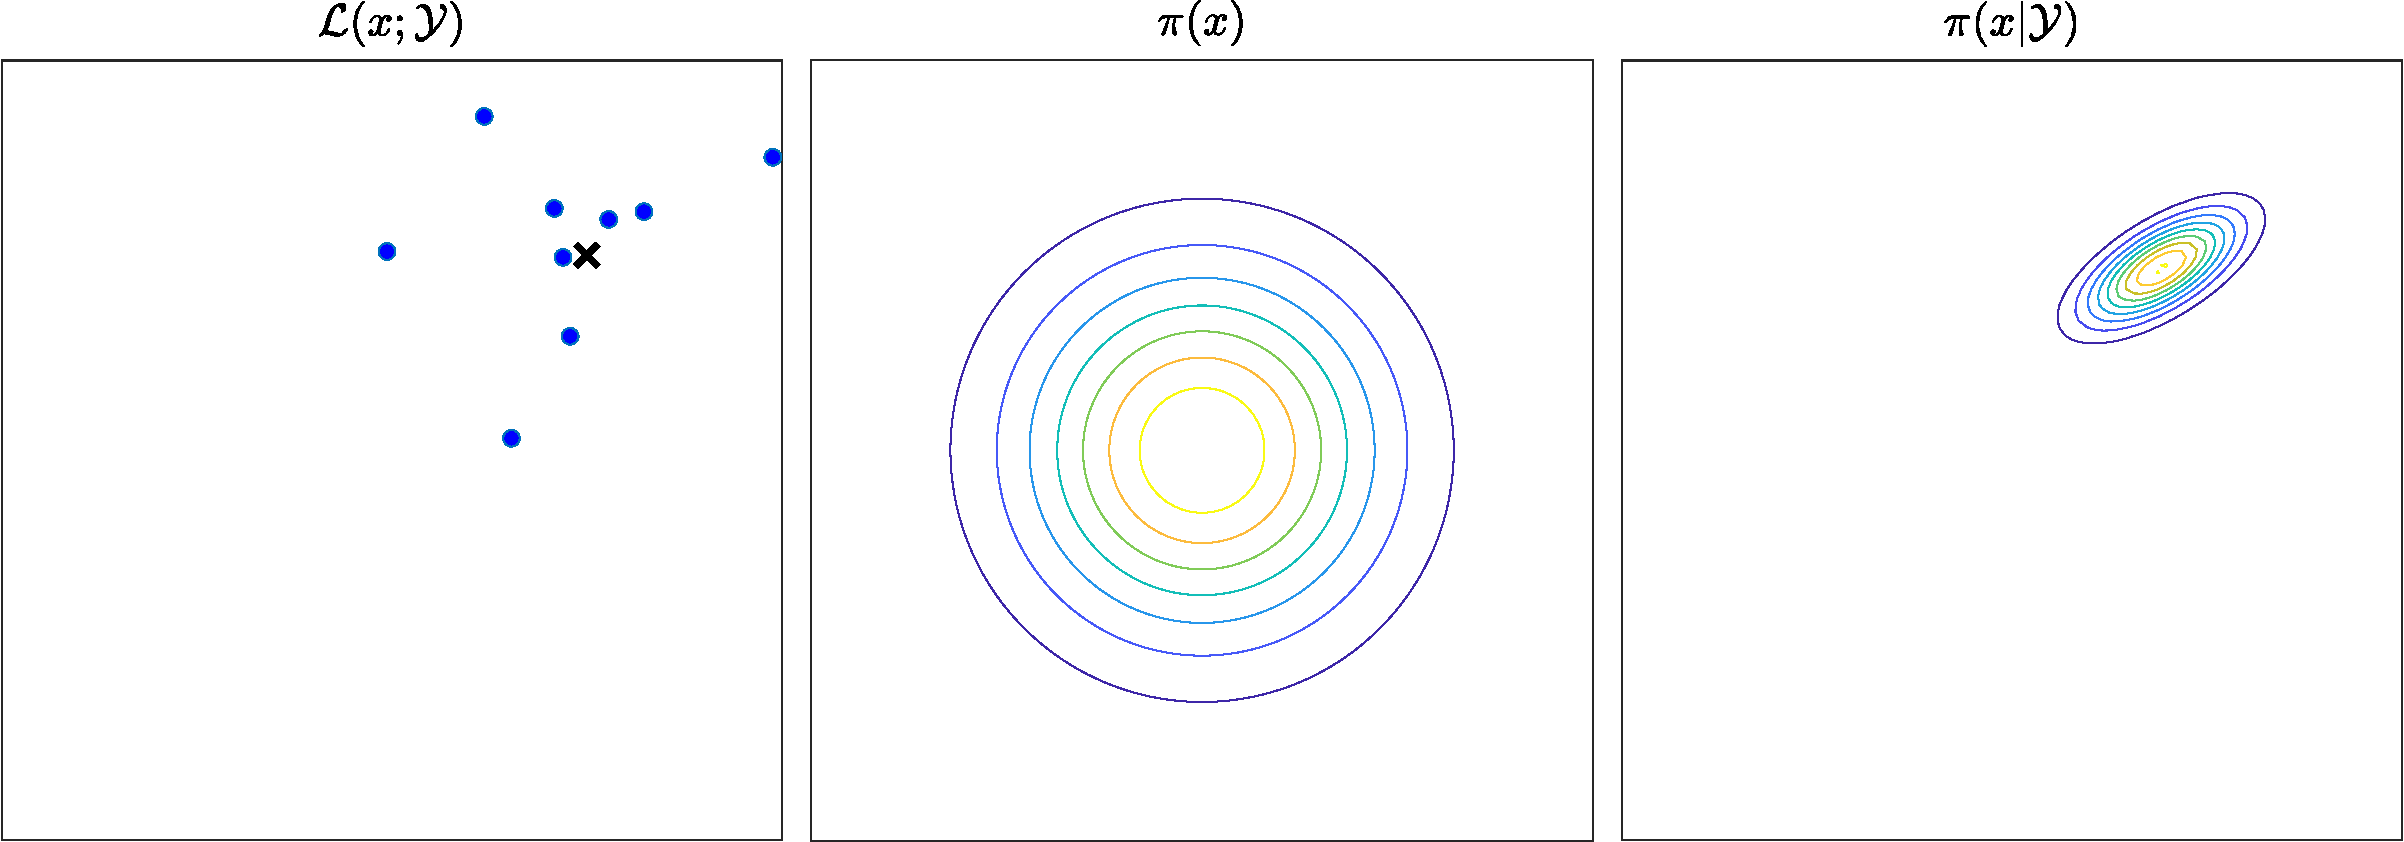
\includegraphics[width = 140mm]{Figures/figure-BI_2D.pdf}
    \caption{Bayesian inference in 2D space}
    \label{fig: BI_2D}
\end{figure}
\section{Posterior quantities of interest}
Under the Bayesian paradigm the posterior distribution $\pi(\boldsymbol{x}|\boldsymbol{y})$ is the solution of the inverse problem. However, in practice it can also serve as an intermediate result that is further processed for interpretation or prediction purpose. Furthermore, the full distribution can contain too much information to allow statements about the inferred parameters. Therefore, it is common to process the posterior and extract certain quantities of interest that summarize the inversion results more concisely.

In many applications, one is only interested in a single parameter $\hat{\boldsymbol{x}}$, i.e., the one that characterise the inversion most suitably. The two most common \textit{point estimation} methods are the posterior mean and \acrlong{MAP} (\acrshort{MAP}). The posterior mean is given as:
\begin{equation}
    \label{eq: posterior mean}
    x^{\rm{mean}} = \mathbb{E}[\boldsymbol{X}|\boldsymbol{Y}] = \int_{\mathcal{D}_{\boldsymbol{X}|\boldsymbol{y}}} 
    x \pi(\boldsymbol{x}|\boldsymbol{y}) {\rm{d}} \boldsymbol{x}    
\end{equation}
It reflects what we expect the parameter value to be after the inference. The \acrshort{MAP} parameter, as the mode of the posterior distribution on the other hand, is the one maximises the posterior




The practical computation of posterior distributions is not trivial, since computing evidence $\pi(\boldsymbol{y})$ is usually not a tractable problem. 


To make the calculation more feasible, we usually choose the \textit{conjugate prior} \citep{gelman1995} to the likelihood, so the integral can be represented analytically. However, in the general cases, sampling methods shall be used.

\section{Exact inference}
\subsection{Variant elimination}
\subsection{Belief propagation}

\section{Approximation inference}

\subsection{Expectation maximization algorithm}

\subsection{Ensemble Kalman filter}
\subsection{Sequential Monte Carlo}
\begin{figure}[htbp]
    \centering
    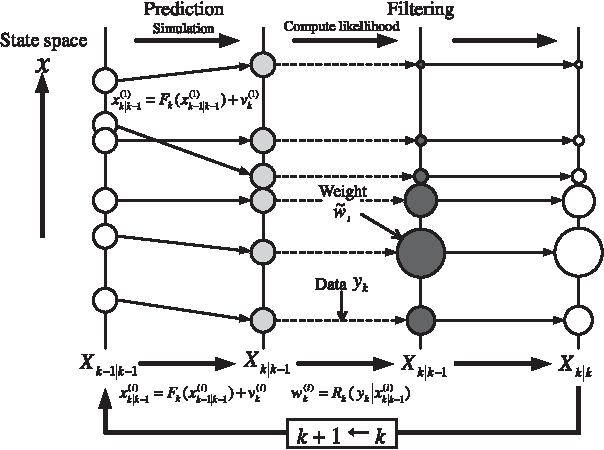
\includegraphics[width = 140mm]{Figures/figure-particle filter.pdf}
    \caption{Bayesian inference in 2D space}
    \label{fig: particle filter}
\end{figure}

\subsection{Markov Chain Monte Carlo}
